\documentclass[nofonts]{ctexart}
%\CTEXsetup[name={Step ,},number={\arabic{chapter}}]{chapter}
\setCJKmainfont[ItalicFont={AR PL UKai CN}]{AR PL UMing CN} %设置中文默认字体
\setCJKsansfont{WenQuanYi Micro Hei} %设置文泉驿正黑字体作为中文无衬线字体
\setCJKmonofont{WenQuanYi Micro Hei Mono} %设置文泉驿等宽正黑字体作为中文打字机字体

\usepackage{amsmath}
%\usepackage{wallpaper}
\usepackage{xcolor}
%\usepackage{pgf, tikz}
\usepackage{multirow}
\usepackage{listings}
\usepackage{color}

\definecolor{keywordcolor}{rgb}{0.8,0.1,0.5}
\definecolor{webgreen}{rgb}{0,.5,0}

%\usepackage[paperwidth=185mm,paperheight=260mm,text={148mm,210mm},left=21mm,includehead,vmarginratio=1:1]{geometry}
%\usepackage[raggedright]{titlesec}
%\titleformat{\chapter}[display]{\Huge\bfseries}{Step \,\thechapter\,}{1em}{}

%\usepackage{fancyhdr}
%\pagestyle{fancy}
%\fancyhf{}
%\fancyhead[ER, OR]{\leftmark}
%\fancyhead[EL, OL]{《编译实习》实习报告}
%\fancyfoot[C]{\thepage}
%\renewcommand{\chaptermark}[1]{\markboth{\thechapter.\ #1}{}}


\lstset{language=C,
basicstyle=\footnotesize,
keywordstyle=\color{keywordcolor}\bfseries, %\underbar,
identifierstyle=,
commentstyle=\color{green} \textit,
stringstyle=\color{red} \ttfamily,
showstringspaces=false,
frame=single,
numbers=left,
numberstyle=\tiny \color{blue},
backgroundcolor=\color{white},
captionpos=b
}


\begin{document}

\title{%
\vspace{-30mm}\Huge NachOS Lab5 实习报告 \vspace{10mm}}
\author{%
\Large 史杨勍惟 
\\[10mm] 1200012741 信息科学技术学院}
\date{2016,05,30}

\maketitle

\newpage
\tableofcontents
\newpage

\section{总体概述}
这次的Lab主要内容是实现文件系统的一些扩展功能。

\section{任务完成列表}
\begin{table}[h]
\footnotesize
\begin{tabular}{|c|c|c|c|c|c|}\hline
\textbf{Exercise 1} & \textbf{Exercise 2} &
\textbf{Exercise 3} & \textbf{Exercise 4} &
\textbf{Exercise 5} & \textbf{Exercise 6}\\\hline
Y & Y & Y & Y & Y & Y\\\hline

\end{tabular}
\begin{tabular}{|c|c|c|}\hline
\textbf{Exercise 7} & \textbf{Challenge 1} & \textbf{Challenge 2}\\\hline
N & N & N\\\hline

\end{tabular}


\end{table}
\section{完成情况}
\subsection*{Exercise 1}
Nachos 的文件系统建立在模拟磁盘上,Nachos 先初始化了 SyncDisk,
是对异步磁盘的一个同步抽象,之后初始化了 FileSystem这个文件系统。Nachos 实现了两种文件系统,一个是基于 unix 本身的文件系统的实现,本次 lab 与之无关, 另一个是实现在 Nachos 模拟磁盘上的文件系统,是这次 lab 的核心。
目前的文件系统只有简单的操作,
构造函数根据参数决定是否建立一个新的文件系统,如果是的话,先生成新的位图和空白的根目录,其
中位图用于管理空闲磁盘的扇区使用情况。接着生成位图 FileHeader 和目录 FileHeader,这里暂时停下
去看 filehdr.h/filehdr.cc 中对 FileHeader 类的定义。

Nachos 的 FileHeader 类有些类似我们在原理课上的 i 结点,给出有关文件的一些属性(目前有文件
大小和占用扇区数), 并用于索引文件(目前只是直接索引),目前,一个文件头恰好占据一个扇区。
Allocate 方法在磁盘上为一个文件分配空间,于是在 filesys.cc 中文件系统初始化中,0 和 1 扇区是存了位
图文件和根目录文件的文件头,然后又进一步为两个文件分配了空间。Deallocate 方法与 Allocate 相对,
是释放对应扇区。另外一对方法 FetchFrom 和 WriteBack 分别将文件头读出/写入磁盘。

回到 filesys.cc 的文件系统初始化部分,此时位图文件、根目录文件空间均已准备好,之后将内容写
回磁盘对应扇区。FileSystem 类还有两个成员方法,Create 方法创建一个文件,实际上与文件系统初始
化中对位图文件/根目录文件的创建类似,只不过这里需要将这个文件加入到根目录中。Open 方法从根
目录中搜索对应文件名,并且打开对应文件。Remove 方法从根目录中搜索对应文件名,并且释放该文件
占用的扇区,同时更新位图文件、根目录文件内容。这些过程中都涉及 OpenFile 类和 Directory 类,下面介绍。

OpenFile 类定义在 openfile.h/openfile.cc 中,是对一个处于打开状态的文件的抽象。打开文件是通
过给出文件头的扇区号索引的,其余成员方法包括我们较为熟悉的文件操作:Seek 将文件指针移到某一
位置,便于随机读写;Read/Write 分别是从文件读入缓存区和从缓冲区写入文件。写操作会通过
SyncDisk 类的方法写入磁盘对应位置。

Directory 类定义在 directory.h/directory.cc 中,是对目录文件的抽象,实质上每一个目录项
(DirectoryEntry)是一个<文件名,文件头扇区>对,当然还有一位表示该目录项。目前支持的基本操作包
括 Add(添加一个文件)、Remove(移除一个文件)和 Find(找到对应文件的文件头位置),因为实际
是对一个二维数组进行操作,实现比较简单。同 FileHeader 类,Directory 类也有 FetchFrom 和
WriteBack,分别将目录文件读出/写入磁盘。Nachos 这一点还是不错的,很注意磁盘与内存的数据结构
上的统一。
\subsection*{Exercise 2 \& Exercise 3}

这个练习很简单,FileHeader 类存储了有关文件的各种属性(除了文件名),因此将新添加的属性全部声明在该类中。
至于扩展文件名长度,我把字符数组换成字符指针。

不过这样做其实是有一定问题的,但是我也无力想到更好的办法。

我一共添加了 type (类型)、 createTime (创建时间)、 accessTime (上次访问时
间)、 modifyTime (上次修改时间)、 path (路径) 5 个 int 变量。给 FileHeader 类增添一个 Init 方法
设置类型( 0 表示文件, 1 是目录)、创建时间( stats->totalTicks )和路径(上级目录扇区号),在 filesys.cc 中的 Create 方法中调用。上次访问时间在 openfile.cc 中的 ReadAt 方法更新,
上次修改时间则在 WriteAt 更新。
对于扩展文件名长度,直接将 char 数组改为 char 指针,长度即不受限。需要在 Add 方法中做修改,
将原来的 strncpy 改为直接赋值。

\subsection*{Exercise 3}

我在 Nachos 全部直接索引的基础之上加入了一级索引。从目前直接索引块中取一些作为一级索引块,这些一级索引块完全不需要存储文件属性之类的东西,只需要存储
直接索引,因此可以存 128/sizeof(int)=32 个直接索引。之前在上个 Exercise 加了一些属性,导致可用
的索引块减为 (128-7*sizeof(int))/sizeof(int)=25 个,我这里取 5 个作为一级索引块,此时总的直接索引
块数变为 20+5*32=180 个,文件大小最大可达 180*128=23040B 。

在实现上,我首先定义一些宏,将一级索引加入。然后,修改几个函数,对于 FileHeader 类的 Allocate
方法,要进行判断,如果请求的扇区块用直接索引即可满足,就仍然维持原状;否则,需要使用一级索引。因为一个一级索引块存储的直接索引块已知,因此此时可以直接算出需要用到几个一级索引,为这些一级索引和对应的直接索引分配扇区。最后注意调用 SynchDisk 类的 WriteSector 方法,将从直接索引指向的扇区的编号写入当前一级索引指向的扇区中。对 Deallocate 方法的修改与 Allocate 很类似,只不过是对于一个一级索引块,需要先用 SynchDisk 的 ReadSector 方法将其中的直接结点的扇区号读出,先将它们释放之后,再释放这个一级索引块。最后修改 ByteToSector 函数,原本的方法可以算出文件的对应扇区,但是现在引入一级索引,需要转换成文件系统上的对应扇区号。


\subsection*{Exercise 4}
为了实现多级目录,我主要设计了 3 个函数。 FindFile 函数是一个基础辅助函数,它接收一个路径
作为参数,然后返回路径对应文件 / 目录的文件头扇区号,其实也就是通过一个路径名找到一个文件 / 目录。
具体地,我采用循环的方式,一个个地读取两个“ /” 之间的字符串,然后在当前目录项中寻找这个文件,
得到其文件头扇区号。举个例子更好一些,比如路径名是“ /a/b”, 其中我定义“ /” 代表 Nachos 文件系统根
目录,进入函数后,首先从根目录表项中找到文件 a ,确认 a 是目录项,然后将当前目录转为 a ,但是这
里并不是改变全局的 directoryFile ,而只是一个临时变量,因此找寻过程并不会真正改变文件系统的当
前目录。然后,再仿照前一步,从 a 目录表项中找到文件 b ,返回 b 文件的文件头扇区号。
下面是主函数之一,创建目录 CreateDirectory ,两个参数分别代表名称和绝对路径,意味着在给定
绝对路径下建立目录,当然绝对路径是一个可选参数,如果不提供的话,意味着在当前目录下进行操作。
这一“名称 + 绝对路径”的模型在多级目录设计中尤为重要,因此后面的删除目录也采取这种模型,另外,
原有的 Create 和 Remove 方法的参数也被修改为这一模型,意味着可以在某一给定路径下新建 / 删除文
件。因为目录也是文件,所以新建目录其实大部分借鉴已有的 Create 方法,只说下不同点。首先,利用
FileHeader 的 Allocate 方法时,因为目录大小是固定的,因此传入参数 DirectoryFileSize 。另外,要
把创建的文件类型标记为“目录”。最后,学习 UNIX 目录项内容,目录项前两项分别是当前目录 (.) 和上
级目录 (..) ,因此我在创建的时候就把这两项加入到新的目录项中去了。虽然现在并没有这么要求,但是
这么做方便以后为 Nachos 设计 Shell 。
删除目录 RemoveDirectory 相对复杂一些,首先利用之前提到的 FindFile 函数得到此目录的文件
头扇区号,从而调整当前目录。然后,对目录项进行遍历,如果碰到一个文件,就直接删除;否则,构
建子目录路径名,传入 RemoveDirectory 进行递归删除。最后,利用 Remove 方法删掉当前目录。

测试代码如下:
\begin{lstlisting}
    fileSystem->CreateDirectory("shiyqw");
    fileSystem->CreateDirectory("OS", "/shiyqw");
    fileSystem->CreateDirectory("Nachos", "/shiyqw/OS");
    fileSystem->Create("Lab4", 1000, "/shiyqw/OS/Nachos");
    fileSystem->Create("Lab5", 1000, "/shiyqw/OS/Nachos");
    fileSystem->Print();
    fileSystem->RemoveDirectory("OS", "/shiyqw");
    fileSystem->Print();
\end{lstlisting}

测试结果正常。

\subsection*{Exercise 5}
当文件被执行写操作导致大小变得比创建文件时的大小大时,需要改变文件的大小。这里我只实现
了增加文件大小的操作,因为这似乎更常用一些。实现这一功能,主要工作实际上都在处理直接索引和
一级索引直接的关系,分情况进行讨论。

实现过程中,
首先,需要在 OpenFile 类的 WriteAt 函数的判断文件大小是否需要增加处加入代码,调用
FileSystem 类下的 ChangeFileSize 函数,它主要是个过渡函数,主要是调用 FileHeader 类的
ChangeSize 函数,只不过在前后加入了对位图的读 / 写。 ChangeFileSize 是关键,它计算出现在文件需要的总扇区个数,然后进行分配。因为之前引入了间接索引,这里需要分几种情况:
\begin{enumerate}
\item 仍然只需要直接索引。很简单,直接分配。
\item 原来不需要一级索引,现在需要了。此时,将剩下的直接索引分配完,然后分配一级索引,过程类似 Allocate 里的分配。
\item 原来也需要一级索引,又有两种情况:
\end{enumerate}

\begin{enumerate}
\item 利用原来的最后一个一级索引中剩下的间接索引,就可以满足新的扇区要求。这样找到原来
的最后一个一级索引号,从上次分配的地方继续分配直接索引。
\item 原来的最后一个一级索引中剩下的间接索引,不能满足新的扇区要求。这样,再将原来一级
索引占满之后,还需要新的一级索引。
\end{enumerate}

最后做了一些测试,仍然利用 fstest.cc 中的函数,狠心一点,把初始文件大小设为 0 ,实际最终文件大小仍是 10KB (因
为执行了 1000 次写 10B 到文件的操作),打印出文件大小增加的信息和最终文件占用索引块的具体信
息,结果如下:
\begin{figure}[h!]
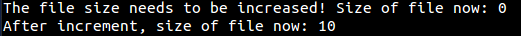
\includegraphics[width=5in]{e51.png}
\end{figure}
每执行一次写文件操作,就会增加一次文件大小,图中显示的是第一次进行了 10B 的写入后,文件
大小从 0 增加到 10B 。
最终结果如下,可以看出,结果和之前完全一样。而且我的测试中,文件大小从 0 到 10KB ,覆盖了我之前讨论的所有情况,因此实现是正确的。
\begin{figure}[h!]
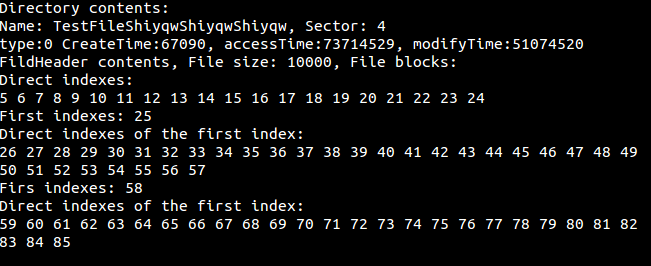
\includegraphics[width=5in]{e52.png}
\end{figure}

\section*{Exercise 6}
\subsection*{代码阅读}
\subsection*{实现}
console.h/console.cc 中的 Console 类是 Nachos 对于终端的模拟,同磁盘相同,系统可以从终端读
/ 写字符,终端本身也是异步的 I/O 设备。由于有了 SynchDisk 类抽象 Disk 类的思路,这里添加两个文
件 synchConsole.h 和 synchConsole.cc ,定义 SynchConsole 类对 Console 类抽象。


实现中,与磁盘相同,终端也有读 / 写操作,只不过 Nachos 将从终端的输入以及显示在终端的输出分成两个
文件模拟,因此,与 SynchDisk 类不同, SynchConsole 类需要为读 / 写操作各自设置一把锁和一个信号
量,以及对应的响应函数。 SynchConsole 类最终设计如下:
\begin{lstlisting}
class SynchConsole {
  public:
    SynchConsole(char *readFile, char *writeFile);
    ~SynchConsole();			
    void PutChar(char ch);	
    char GetChar();	   	
    void WriteDone();	 	
    void CheckCharAvail();

  private:
    Console *console;
    Semaphore *writeSemaphore;
    Semaphore *readSemaphore;
    Lock *putLock;
    Lock *getLock;
};

\end{lstlisting}
然后,对于每一种操作,几乎是对 SynchDisk 类的操作的实现如出一辙,都是在函数头尾加锁 / 解锁
防止其他线程进入,然后利用信号量的 P 操作使线程等待直到等待事件完成,使用信号量 V 操作被唤醒。
不同的一点是,对于读终端操作, Nachos 现有实现是每个一段事件询问终端是否有字符输入,有的话产
生中断,因此对于 SynchConsole 的读操作,是先利用 P 操作让线程等待,然后当检测到字符时使用 V
操作唤醒。写终端操作恰好相反,是先进行写操作,然后等待动作完成被唤醒。

以下为测试结果,可以看到我我按下回车Console会显示我输入的字符串。没有则会进入忙等。
\begin{figure}[h!]
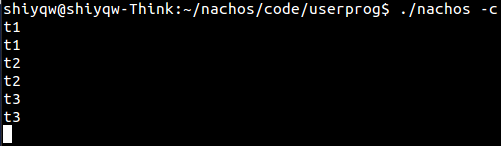
\includegraphics[width=5in]{e6.png}
\end{figure}


\section{遇到的困难以及解决办法}
遇到的主要困难在于时间不够,由于这两个Lab本身都只有一周的时间,又适逢毕业设计,所以时间实在是不够。虽说我认为这个Lab的难度应该是小于Lab4的,不过代码量也不小,我最终Exercise7也没有完成,希望面测之前能够补完这些代码。

\section{收获与感想}

收获在于对文件系统有了更深入的认识,其实文件系统和之前的部分总让人感受到有一种脱离的感觉,好像这块部分和其他部分的关系不大。不过做了这个Lab,我也深刻地感受到了文件系统和其他部分也是有关联的,比如和进程管理和虚拟内存之间那种千丝万缕的关系。

这次Lab我真的是水过了,包括下一个Lab,只是初步地完成了实现。

\section{意见与建议}
无。

\section{参考资料}
\begin{itemize}
\item 《现代操作系统》
\end{itemize}

\end{document}